\section{Data Integration and Assimilation Systems}
\label{se:dias}

\acrfull{dias} \cite{Kawasaki2018DataReduction} collects and archives data from satellites, weather stations, numerical forecasting models and climate projection models. Once this data is integrated into geographic useful information, DIAS generates results for managing global environmental problems and natural disasters \cite{Kawasaki2018DataReduction}. As mentioned above, \acrshort{dias} has the capability of collecting weather data from multiple data sources which are inherently in different formats. After successfully ingest the data, it generates results which can use for different kind of purposes.

\begin{figure}[htp]
    \centering
    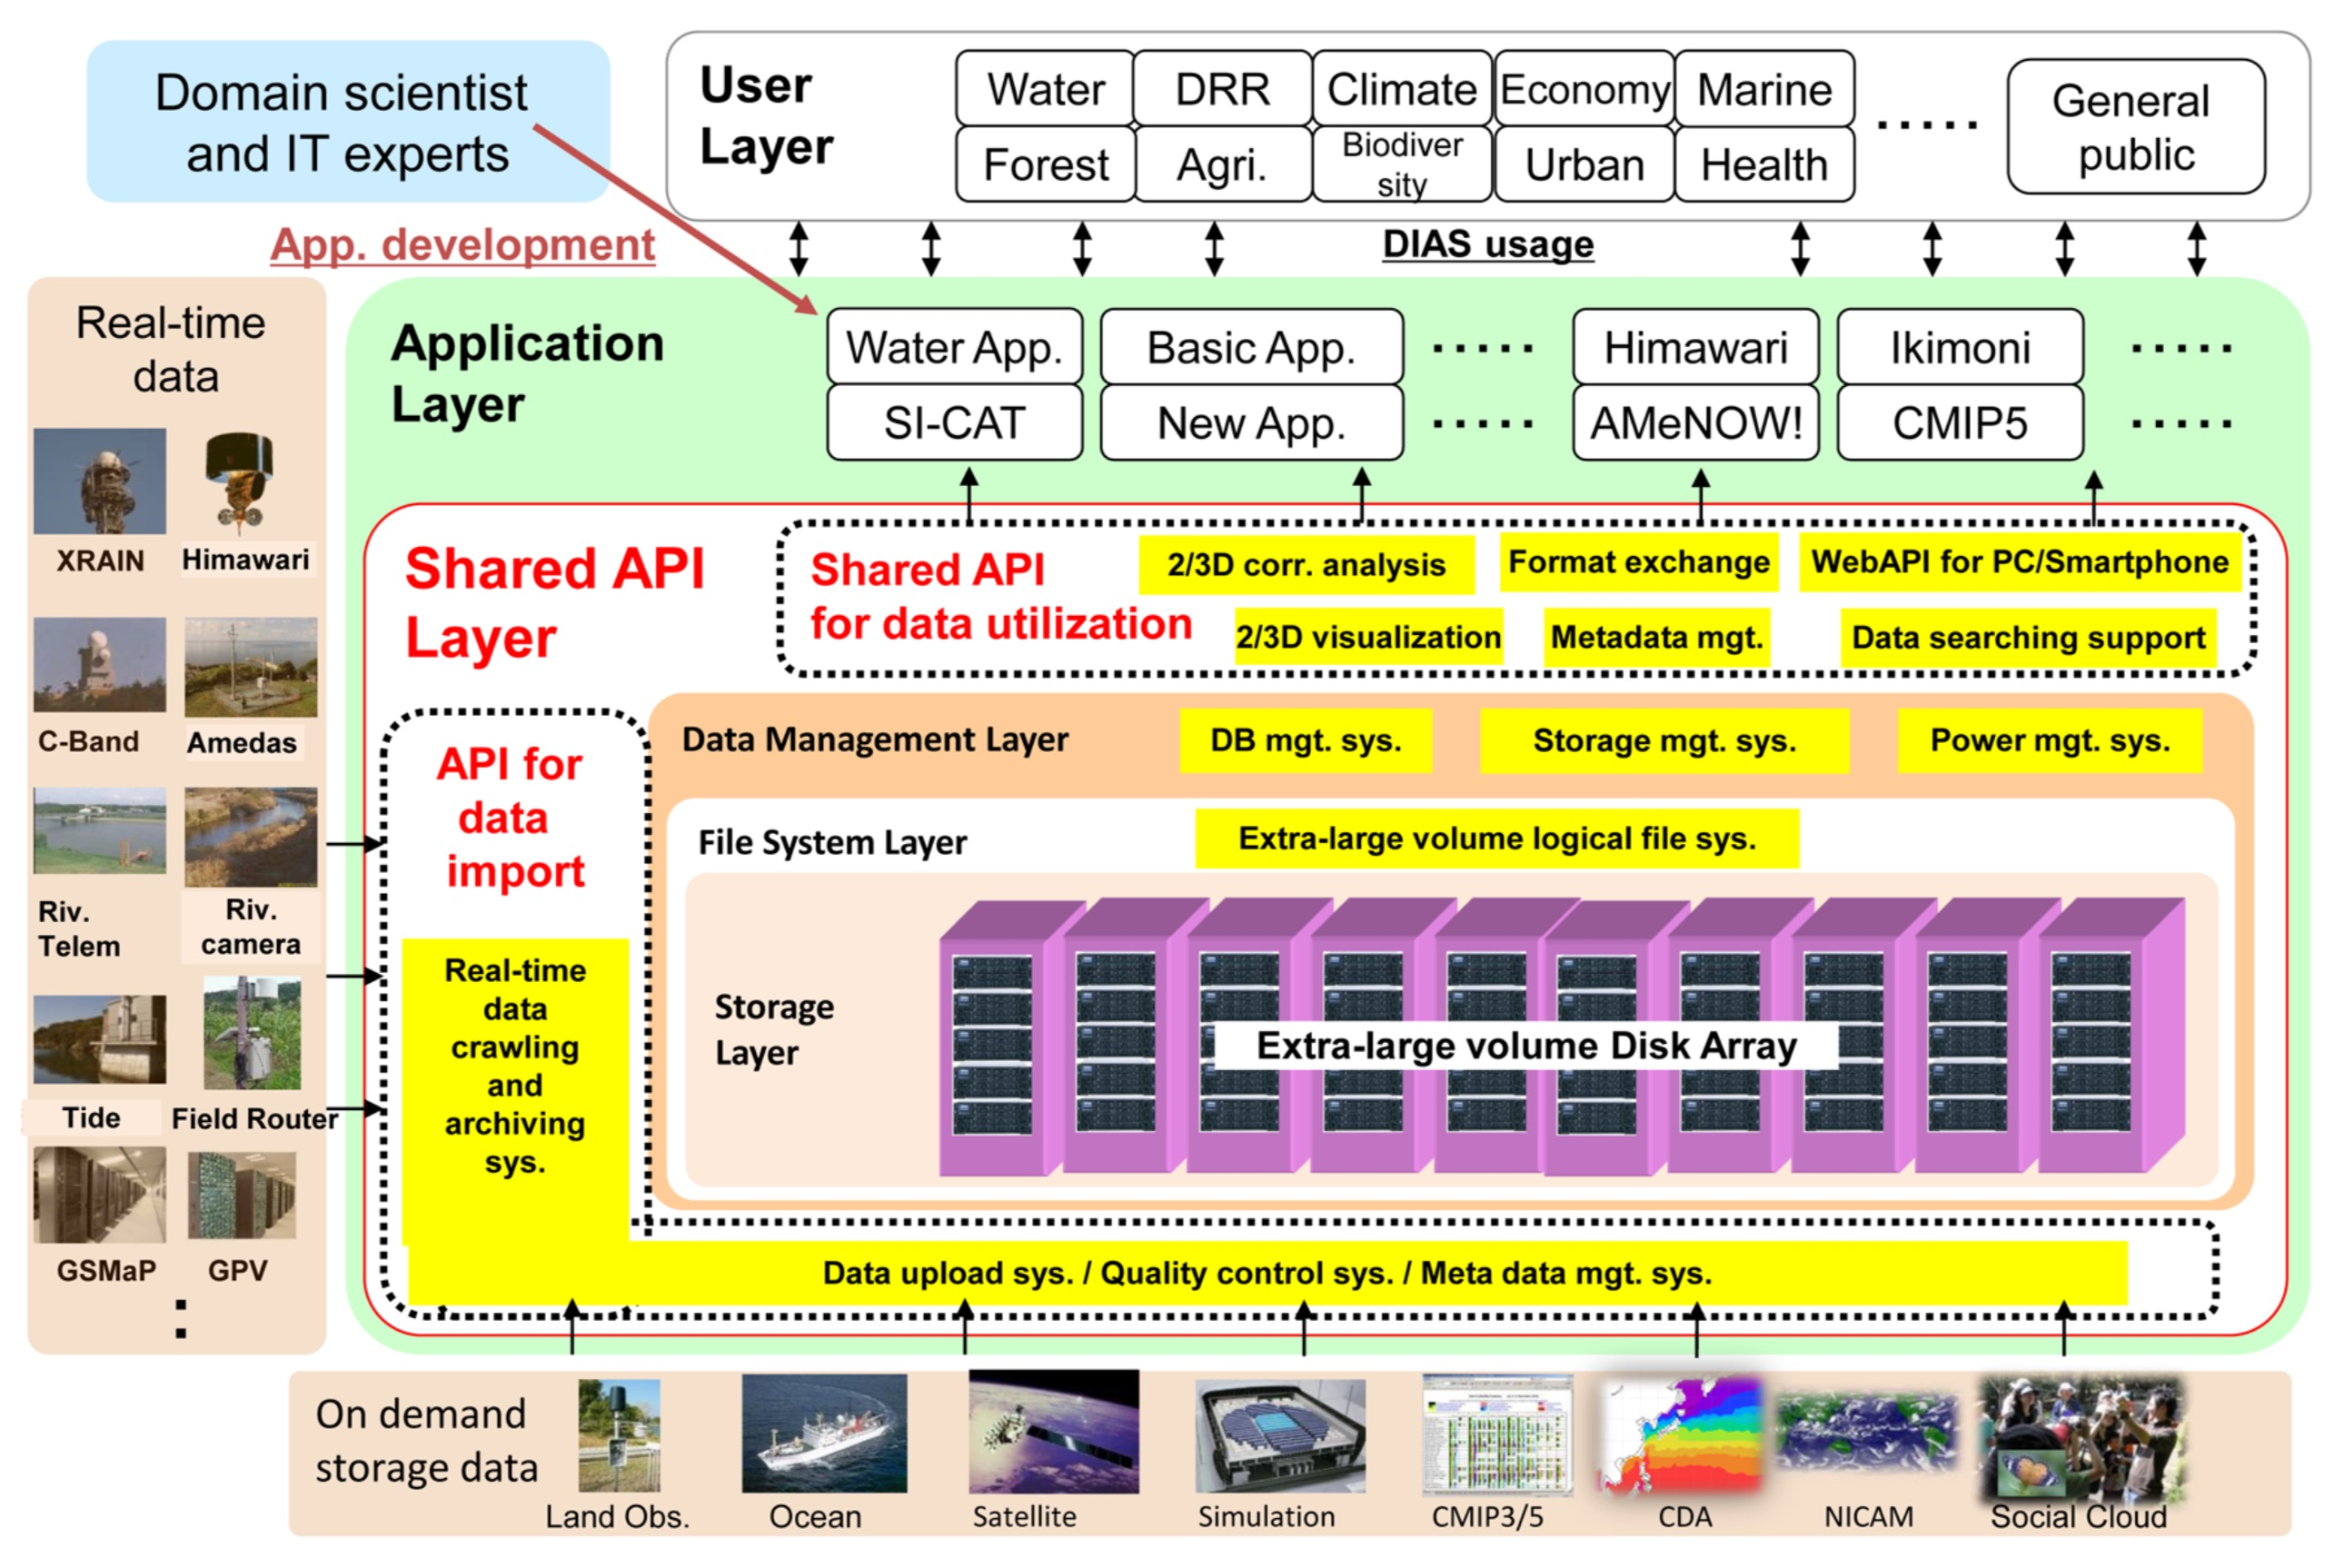
\includegraphics[width=1\textwidth]{lit/other/dias_common_base_application_platform.jpg}
    \caption[DIAS’s common base application platform.]{DIAS’s common base application platform \cite{Kawasaki2018DataReduction}.}
    \label{fi:dias_common_platform}
\end{figure}

The mechanism of storing data in \acrshort{dias}, similar to the other systems discussed.
These data sets are stored in a larger array system with API software that is used to import the data. APIs work to convert or reformat data into manageable forms and are useful for creating the DIAS storage archive. The API software contains various tools, including the real-time data exploration and archiving system, the data download system, the quality control system and the metadata management system \cite{Kawasaki2018DataReduction}. To store on the large volume of disk space, it converts the data via a provided set of APIs. This can be considered the same as the open data model provided by the \acrshort{fews}. Other than that, \acrshort{dias} consist of additional tools that provide the functionality of quality control of the data, and metadata management which is similar to some of the services in \acrshort{lead}.

As shown in \cref{fi:dias_common_platform}, it offers an application layer that allows scientists in the field to work on research tasks and to develop specific tools and applications by collaborating with experts in information technology \cite{Kawasaki2018DataReduction}. Once the data is achieved on the \acrshort{dias} system, it shares those details via the Shared API layer. Thus it allows users to remote access to the data, and easy integration via the APIs.



%%%%%%%%%%%%%%%%%%%%%%%%%%%%%%%%%%%%%%%%%%%%%%%%%%%%%%%%%%%%%%%%%%%%%%%%%%%%%%%%
\section{Meteorological Assimilation Data Ingest System}
\label{se:madis}
\acrfull{madis} \cite{Macdermaid2005ArchitectureP2.39} is a data integration and assimilation system that collects data from dozens of suppliers, then checks the quality of the data and saves it in \acrshort{netCDF} format. Give users later access to data through support for different types of protocols.

\dbc{Both MADIS and netCDF need to cited. Do this at the beginning for each on the systems in this chapter (while they were cited in Chap 1, it's also important to cite them in Chap 2 as well.}
\gkc{Updated.}

\begin{figure}[htp]
    \centering
    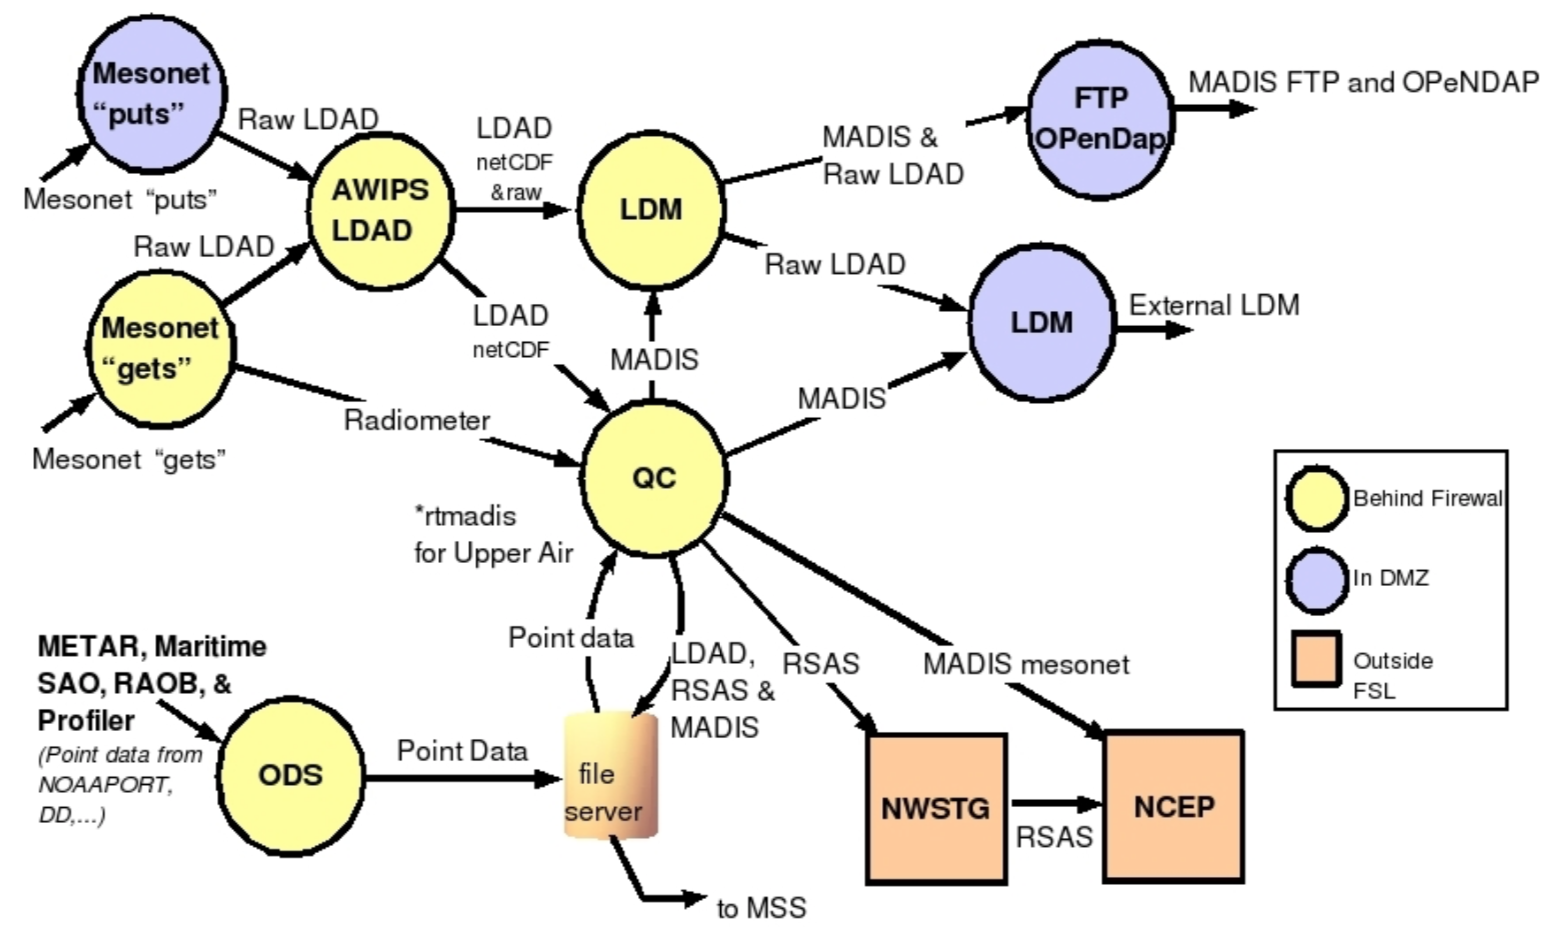
\includegraphics[width=1\textwidth]{lit/other/madis_flow.png}
    \caption[\acrshort{madis} data flow]{\acrshort{madis} data flow \cite{Macdermaid2005ArchitectureP2.39}.}
    \label{fi:madis_flow}
\end{figure}


\acrshort{madis} contains a distributed architecture for data acquisition, processing and distribution functions.
In addition, the paper mentioned architectural advancement at that time, the various functional hosts have been paired using Linux High Availability (HA) to provide automated failover in the event of a system failure. And it uses following method for data dissemination such as FTP, Local Data Manager (LDM) and the Web OPeNDAP (OPen source project for Network Data Access Protocol) \cite{Macdermaid2005ArchitectureP2.39}. As mentioned above, the \acrshort{madis} is implemented based on a distributed architecture that is available at the time of its development. Even it is not mentioned, it is using functional calls like Remote Procedure Call (RPC) to invoke among a cluster of nodes. In \cref{fi:madis_flow}, data is transported from the input and preprocessing systems to the central computer systems and then to other hosts for storage and distribution \cite{Macdermaid2005ArchitectureP2.39}. To get high availability, it has added some updates to its architecture as mentioned in the paper. The conclusion of this statement is, these kinds of functionalities are available at the modern the Cloud Computing tools, and out of the box, those tools are providing the scalability and high availability. Using those tools, it possible to implement such a system with less effort and high confidence.

MADIS regularly acquires Mesonet data from dozens of network providers representing more than 14,000 stations. This translates into more than 30,000 station reports every hour. Different systems that work inside and outside the firewall collect the data. This data is sent to the data server of the Advanced Weather-Interactive Processing System (AWIPS) of the central installation for processing and conversion to a common format, NetCDF. NetCDF files are then transferred to MADIS compute nodes \cite{Macdermaid2005ArchitectureP2.39}. This provides an overview of the level of data that \acrshort{madis} handling. This could be a good reference for implementing \acrshort{wdias} and its performance testing. As same as \acrshort{fews}, it is also converting the data into a common format which is \acrshort{netCDF}. Those files are transferred to the compute nodes and allow users to access via OPeNDAP. 
%MADIS computer platforms include Intel-based servers with the Red Hat Enterprise Linux operating system. 
Many of these computers are configured using Linux clustering with high availability \cite{Macdermaid2005ArchitectureP2.39}.% As indicated above, the system heavily depends on the platform. There are some costs involving purchasing their licenses.

As certain MADIS data is considered to be the property of the supplier, access to this data must be checked. To respond to this, MADIS data is divided into six different versions, depending on the access level authorized by the data provider \cite{Macdermaid2005ArchitectureP2.39}. When compared to \acrshort{fews}, \acrshort{madis} provides control based access to the data.



%%%%%%%%%%%%%%%%%%%%%%%%%%%%%%%%%%%%%%%%%%%%%%%%%%%%%%%%%%%%%%%%%%%%%%%%%%%%%%%%
\section{Summary}
\label{se:lit_summary}
\db{We presented several related work on WDIA system implementations such as \acrshort{fews}, \acrshort{lead}, \acrshort{dias}, and \acrshort{madis}}. In this research one of major issue that we focused on storing data which are ingested from different sources with different formats efficiently. The \acrshort{fews} and \acrshort{madis} are using the \acrshort{netCDF} as the common data format to store the data which is one of the best solutions available with modern technologies as well. Even it is not mentioned, the \acrshort{dias} and \acrshort{lead} also following a method of having common storage space to store bulk data.
\acrshort{fews} and \acrshort{lead} have the capability of handling the workflow of forecasting, but other systems are mainly focused on providing a weather data management system.
\acrshort{fews} provides a modular approach via its general adapter, and according to the \acrshort{soa} architecture of \acrshort{lead} provides the same functionality via services.
\dbc{Complete highlighted sentence}
\gkc{Updated. Do I need to elaborate more?}

Most of the above systems developed by many developers and researchers, and were developed specifically to address issues like natural disasters. To address use cases such as CUrW, it required to remodel the systems  and define the forecasting flows. Even some of the systems try to follow a generic approach to integrate new modules, it is challenging to deploy modules for a closed source or proprietary software. Further, most of them are depend on the underline platform, and does not support more resource efficient and highly-scalable technologies such as cloud computing.

\dbc{You are making lots of mistakes when using "ing" form of a verb. It seems checking with Grammaly didn't help either.}
\gkc{I fixed all the issues one by one which are shown by Grammarly free version. Can you highlight with a specific example. I'll add more effort to improve.}
